\section{Discrepancy Audit: 71,320 vs 13,941 Elements and Governing Decision}
\label{sec:discrepancy_audit_71k_vs_14k}

\subsection{Publication Discrepancy and Comprehensive Investigation}
\citet{pandey2025} report an adapted Mode-I element count of $\approx 13{,}941$, while strictly applying the published Listing~1 settings to the full domain generates $71{,}320$ finite elements.

An exhaustive numerical and software investigation established:
\begin{enumerate}
  \item \textbf{Abaqus Release Invariance:} Abaqus 2019 GA, 2021.HF26, 2022 GA, and 2023.HF4 all generate $100.000\%$ bitwise identical $71{,}320$-element meshes with matching SHA-256 hashes.
  \item \textbf{Single-Factor Parameter Testing:} Testing load magnitude, output frequency, boundary conditions, and mesher controls ruled out trivial parameter differences.
  \item \textbf{Regional Breakdown:} The crack process corridor ($|y| \le 0.05\,\mathrm{mm}$) contains $9{,}061$ elements ($12.7\%$), while far-field and transition regions contain $62{,}259$ elements ($87.3\%$) because coarsening was disabled (\texttt{coarseningFactor=NOT\_ALLOWED}).
  \item \textbf{Pre-Analysis Loading and Step Lineage:} Evaluating native remeshing against the qualified two-step layered UEL/UMAT pre-analysis (Job \texttt{1409554.mmaster02}) deterministically yields $48{,}329$ finite elements ($48{,}093$ nodes) under $1.0\%$ error target ($100.000\%$ mesh identity across independent repeats). An interim provisional run (Job \texttt{1409546.mmaster02}) yielded $42{,}318$ elements.
\end{enumerate}

\subsection{Supervisor Decision and Definitive Closure}
During the meeting on 17 September 2026, the supervisor formally closed this investigation under the following governing ruling:
\begin{center}
  \textbf{\texttt{SUPERVISOR\_ACCEPTED\_REPRODUCTION\_LIMITATION\_CLOSED}}
\end{center}
The supervisor confirmed that:
\begin{itemize}
  \item The complete author code, internal scripts, and exact frame selection routines are unavailable;
  \item The publication does not disclose sufficient information to reproduce the specific $13{,}941$ element count;
  \item The reproducible $48{,}329$-element mesh is classified as \textbf{\texttt{PROJECT\_REPRODUCIBLE\_STEP1\_1PCT\_RESULT}}, not an authoritative literature match;
  \item The remaining difference between $48{,}329$ and $13{,}941$, along with the exact step/frame filtering semantics, is formally designated as \textbf{\texttt{UNRESOLVED\_PUBLICATION\_IMPLEMENTATION\_DETAIL}} and \textbf{\texttt{FRAME\_SELECTION\_SEMANTICS\_UNRESOLVED}};
  \item Exact $13{,}941$ reproduction is \textbf{not an active blocker};
  \item Reproduction of general error-guided adaptivity trends is fully sufficient;
  \item Additional effort aimed solely at discovering an unpublished detail is not justified;
  \item All tested sensitivity results shall be preserved in the thesis as documented evidence.
\end{itemize}

\subsection{Preserved Parametric Sensitivity Trends}
Table~\ref{tab:error_target_sensitivity_pack} summarizes the preserved sensitivity results across four target error tolerances, demonstrating monotonic mesh reduction as tolerance relaxes.

\begin{table}[htbp]
\centering
\caption{Parametric sensitivity of adapted finite element counts to the \texttt{errorTarget} tolerance.}
\label{tab:error_target_sensitivity_pack}
\begin{tabular}{lrrrl}
\toprule
Case & \texttt{errorTarget} & Coarse Baseline Count & Corrected Pre-Analysis Count & Classification \\
\midrule
$A_1$ & $1.0\%$ & $71{,}320$ & $48{,}329$ & Reproducible Step-1 1\% result \\
$A_2$ & $2.0\%$ & $17{,}687$ & $11{,}737$ & $2.0\%$ error tolerance \\
$A_3$ & $3.0\%$ & $8{,}120$ & $5{,}158$ & $3.0\%$ error tolerance \\
$A_4$ & $5.0\%$ & $4{,}356$ & $3{,}763$ & $5.0\%$ error tolerance \\
\bottomrule
\end{tabular}
\end{table}

\subsection{Influence of errorTarget on the Final Stage-14 Step-2 Adaptive Refinement}
\label{sec:step2_errortarget_sensitivity}

To systematically establish the spatial localization and element-count sensitivity of the native Abaqus \texttt{adaptiveRemesh} engine when evaluated on the true localized phase-field damage state, a rigorous parametric sweep across $\texttt{errorTarget} \in \{1.0\%, 2.0\%, 3.0\%, 5.0\%\}$ was conducted targeting \texttt{Step-2} ($u_y = 0.010\,\mathrm{mm}$, Frame 1022) of the companion pre-analysis ODB (\texttt{PK\_M1\_JOB1\_INF\_COMPANION\_2906.odb}). All sizing parameters were kept identical ($h_{\min} = 1.0\,\mu\mathrm{m}$, $h_{\max} = 20.0\,\mu\mathrm{m}$, \texttt{refinementFactor = 10}, \texttt{coarseningFactor = NOT\_ALLOWED}, \texttt{region = ALL\_ELEM}).

\begin{figure}[htbp]
\centering
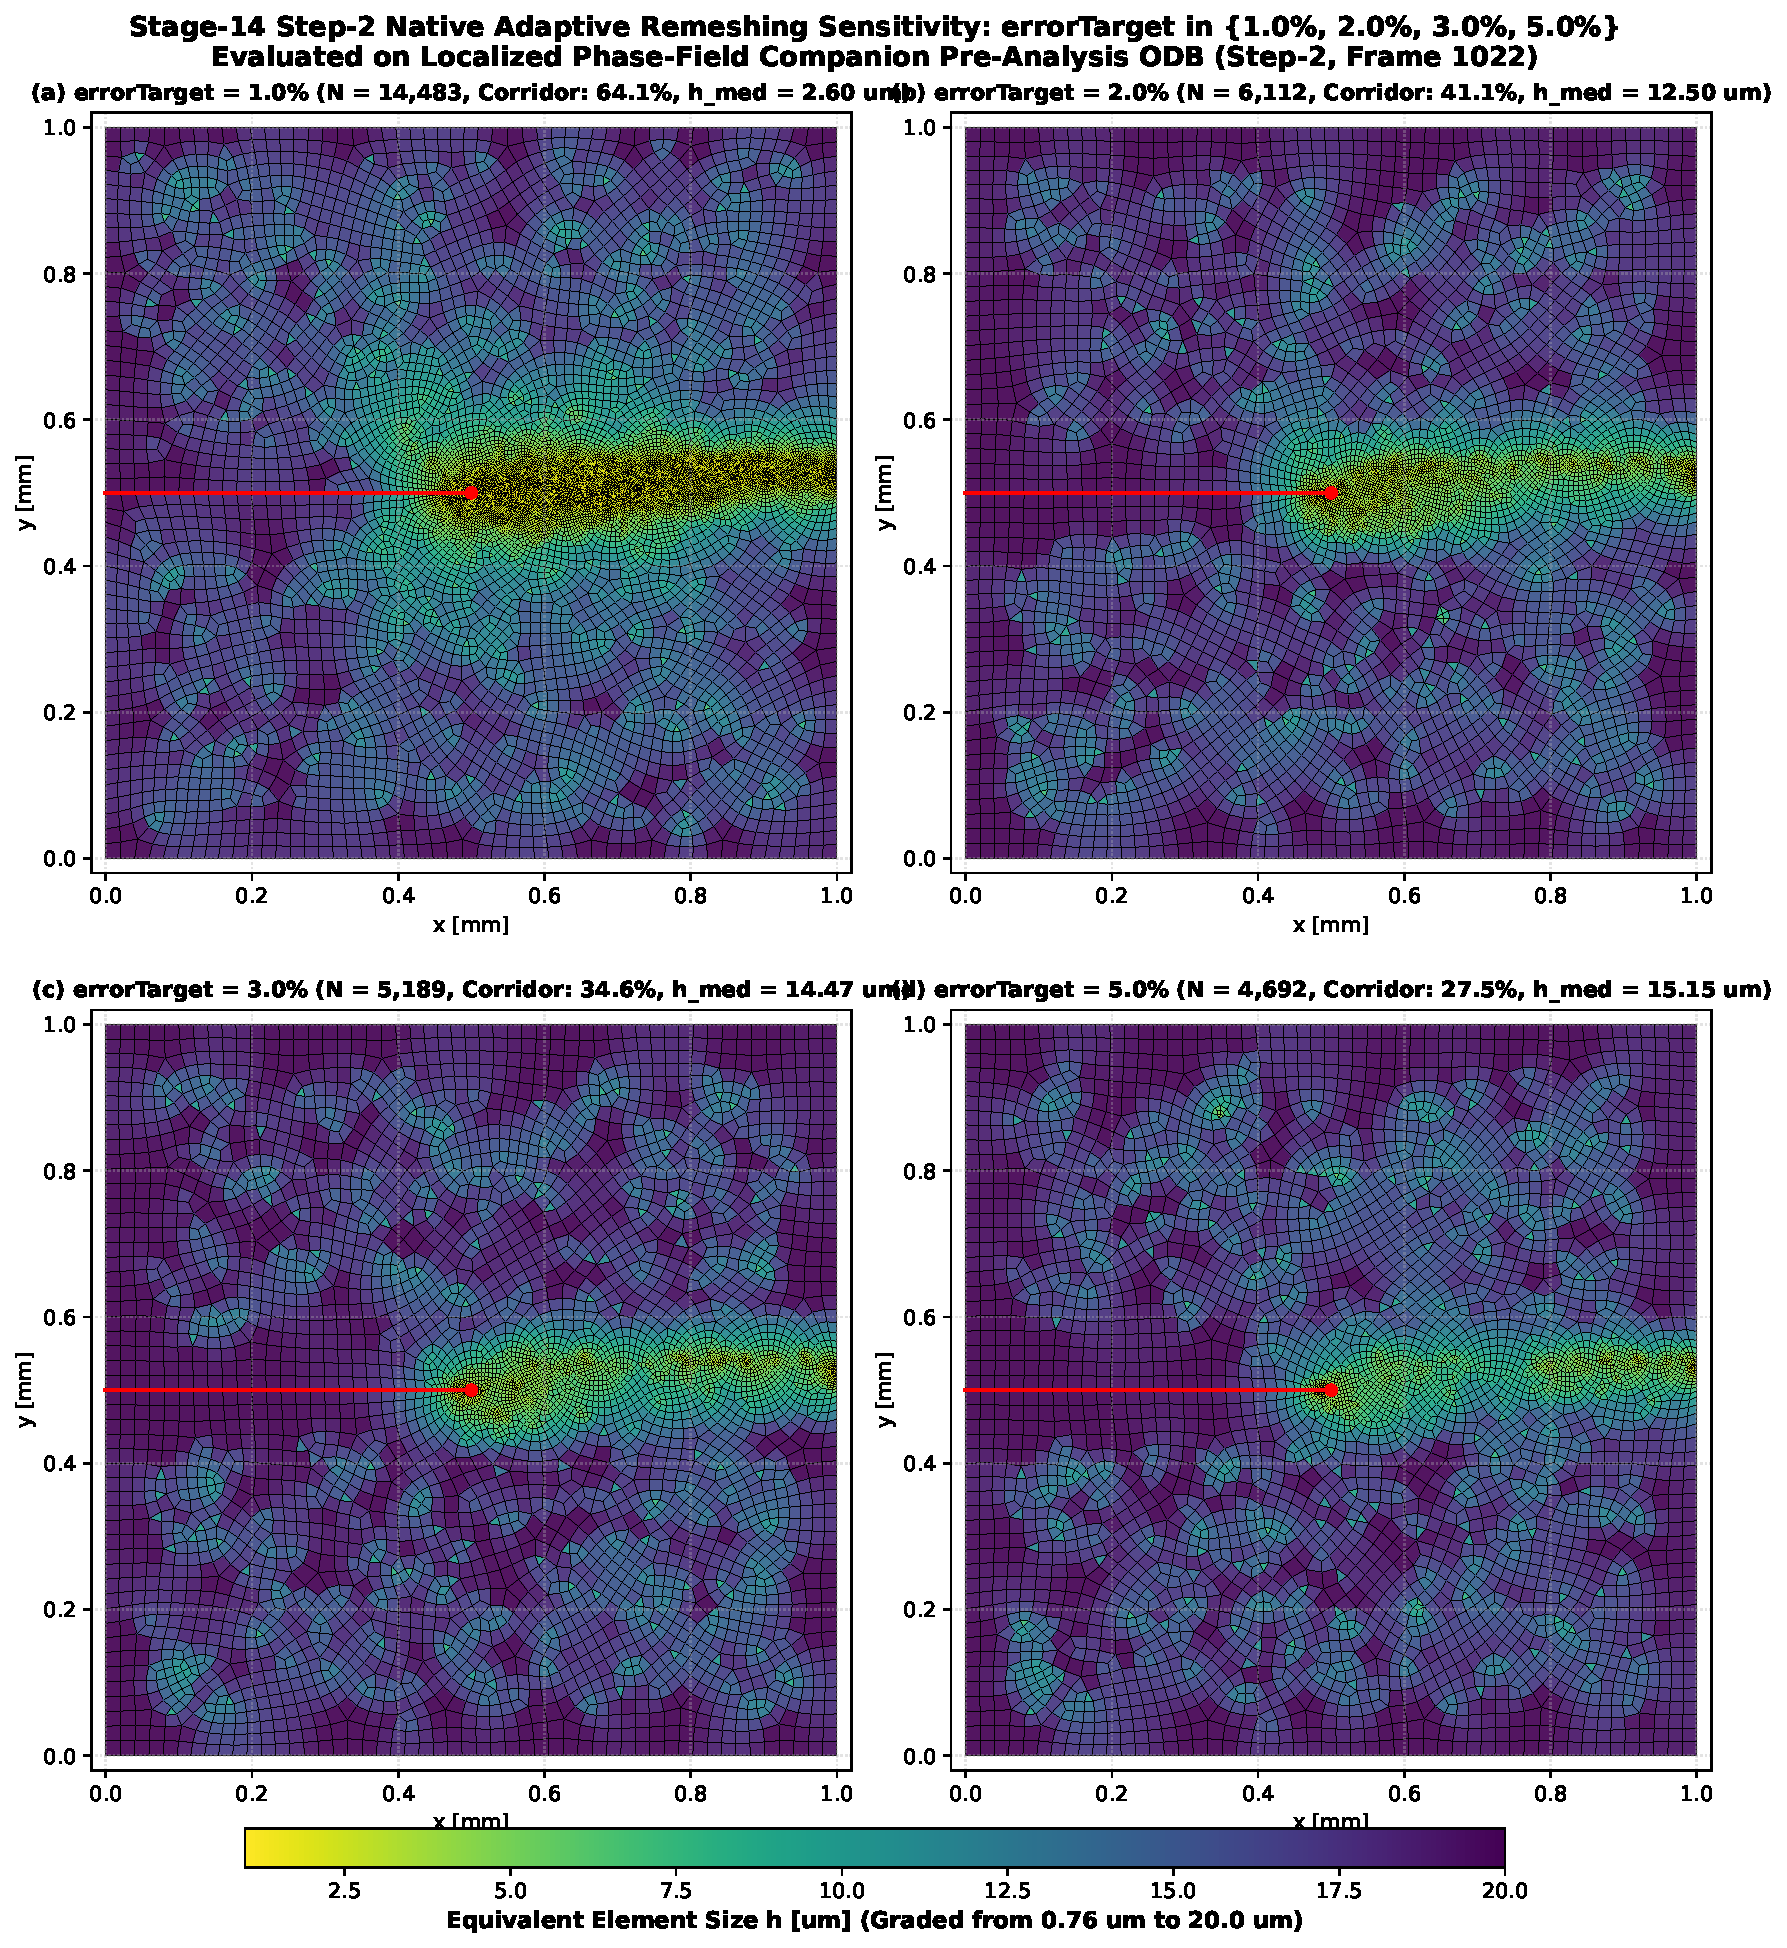
\includegraphics[width=\textwidth]{figures/fig_stage14_step2_errortarget_comparison.pdf}
\caption{Parametric sensitivity of native Abaqus \texttt{adaptiveRemesh} across four error targets ($\texttt{errorTarget} \in \{1.0\%, 2.0\%, 3.0\%, 5.0\%\}$) evaluated on the localized Stage-14 Step-2 phase-field pre-analysis ODB. Color contours depict equivalent element size $h_{\mathrm{eq}} \in [0.76, 20.0]\,\mu\mathrm{m}$. ET1 retains dense, target-like crack-ligament refinement ($64.12\%$ corridor share), whereas ET2, ET3, and ET5 progressively under-refine the horizontal propagation path.}
\label{fig:step2_errortarget_comparison}
\end{figure}

Table~\ref{tab:step2_error_target_sensitivity} presents the quantitative metrics across the four evaluated error targets.

\begin{table}[htbp]
\centering
\small
\caption{Quantitative spatial and morphological metrics for the Stage-14 Step-2 native adaptive remeshing sensitivity sweep.}
\label{tab:step2_error_target_sensitivity}
\begin{tabular}{lrrrr}
\toprule
Metric / Dimension & ET1 ($1.0\%$) & ET2 ($2.0\%$) & ET3 ($3.0\%$) & ET5 ($5.0\%$) \\
\midrule
Total Finite Elements ($N$) & $\mathbf{14{,}483}$ & $6{,}112$ & $5{,}189$ & $4{,}692$ \\
Total Nodes ($N_{\mathrm{nodes}}$) & $\mathbf{14{,}456}$ & $6{,}181$ & $5{,}262$ & $4{,}759$ \\
Element Breakdown (Quads / Tris) & $14{,}082$ / $401$ & $5{,}929$ / $183$ & $5{,}023$ / $166$ & $4{,}522$ / $170$ \\
Corridor Elements ($|y-0.5| \le 0.05\,\mathrm{mm}$) & $\mathbf{9{,}286}$ ($\mathbf{64.12\%}$) & $2{,}510$ ($41.07\%$) & $1{,}795$ ($34.59\%$) & $1{,}291$ ($27.51\%$) \\
Ligament Elements ($x \ge 0.5\,\mathrm{mm}$) & $8{,}325$ & $2{,}063$ & $1{,}465$ & $1{,}022$ \\
Wake Elements ($x < 0.5\,\mathrm{mm}$) & $961$ & $447$ & $330$ & $269$ \\
Far-Field Elements ($|y-0.5| > 0.05\,\mathrm{mm}$) & $5{,}197$ ($35.88\%$) & $3{,}602$ ($58.93\%$) & $3{,}394$ ($65.41\%$) & $3{,}401$ ($72.49\%$) \\
Coarse Area Fraction ($h \ge 15\,\mu\mathrm{m}$) & $59.39\%$ & $75.77\%$ & $78.14\%$ & $77.39\%$ \\
$h_{\min}$ [$\mu\mathrm{m}$] & $0.760$ & $0.956$ & $1.339$ & $1.230$ \\
$h_{\mathrm{median}}$ [$\mu\mathrm{m}$] & $2.597$ & $12.496$ & $14.469$ & $15.151$ \\
$h_{\mathrm{mean}}$ [$\mu\mathrm{m}$] & $6.025$ & $11.174$ & $12.558$ & $13.631$ \\
$h_{\max}$ [$\mu\mathrm{m}$] & $23.020$ & $23.407$ & $23.402$ & $23.319$ \\
Flank Refinement $w(0.1\text{--}0.3)$ [mm] & $\mathbf{0.000}$ & $\mathbf{0.000}$ & $\mathbf{0.000}$ & $\mathbf{0.000}$ \\
Crack Tip Width $w(0.5)$ [mm] & $0.121$ & $0.090$ & $0.079$ & $0.051$ \\
Ligament Width $w(0.6)$ [mm] & $0.170$ & $0.104$ & $0.099$ & $0.021$ \\
Ligament Width $w(0.7)$ [mm] & $0.121$ & $0.074$ & $0.023$ & $0.000$ \\
Ligament Width $w(0.8)$ [mm] & $0.116$ & $0.058$ & $0.055$ & $0.031$ \\
Ligament Width $w(0.9)$ [mm] & $0.077$ & $0.023$ & $0.029$ & $0.037$ \\
Scientific Classification & \textbf{\texttt{TARGET\_LIKE}} & \textbf{\texttt{AWAY\_FROM\_TARGET}} & \textbf{\texttt{AWAY\_FROM\_TARGET}} & \textbf{\texttt{AWAY\_FROM\_TARGET}} \\
\bottomrule
\end{tabular}
\end{table}

\subsubsection{Key Physical and Epistemological Insights}
\begin{enumerate}
  \item \textbf{Exact Stage-14 Mesh Reproduction:} At $\texttt{errorTarget} = 1.0\%$, the native remesher exactly reproduces $14{,}483$ finite elements and $14{,}456$ nodes, bitwise and topologically identical to the Stage-14 Step-2 native remesh artifact (\texttt{PK\_M1\_STAGE14\_STEP2\_ALLINC.inp}, Package 99).
  \item \textbf{Corridor Desensitization Mechanism:} As $\texttt{errorTarget}$ increases from $1.0\% \to 5.0\%$, the corridor element share drops monotonically from $64.12\% \to 27.51\%$. The scientific cause of classification \texttt{AWAY\_FROM\_TARGET\_LOCALIZATION} for ET2, ET3, and ET5 is the progressive loss of spatial resolution across the regularized damage zone ($l_0 = 7.5\,\mu\mathrm{m}$) along the crack ligament, not merely the reduced global element count.
  \item \textbf{Wake Cleanliness Invariance:} Across all four error targets, the initial slit flank ($x \le 0.3\,\mathrm{mm}$) exhibits strictly zero artificial refinement ($w = 0.00\,\mathrm{mm}$), proving that the Step-2 localized damage formulation completely avoids spurious wake remeshing.
  \item \textbf{Lineage Separation:} This Step-2 target-like sweep is strictly distinct from the historical Step-1 linear-elastic sweep ($57{,}929 / 14{,}677 / 6{,}824 / 4{,}239$ elements), which was evaluated before phase-field damage localization occurred.
  \item \textbf{3-Layer UEL Fracture Batch Execution (Jobs 1410357, 1410358, 1410359):} To determine whether the relaxed corridor refinement in ET2 ($6{,}112$ FE), ET3 ($5{,}189$ FE), and ET5 ($4{,}692$ FE) produces a converged mechanical and energetic fracture solution, deterministic 3-layer UEL/UMAT input decks were reconstructed using the verified property cards ($l_0=0.0075\,\mathrm{mm}, G_c=0.0027\,\mathrm{kN/mm}, E=210\,\mathrm{GPa}, \nu=0.3, k=10^{-7}, N_{\mathrm{base}}$), qualified via preflight Abaqus datachecks (Exit 0), and submitted to PBS on \texttt{/scratch9/} under serial 1-CPU execution (Jobs \texttt{1410357.mmaster02}, \texttt{1410358.mmaster02}, \texttt{1410359.mmaster02}).
\end{enumerate}



\subsubsection{Predeclared Fracture Evaluation Matrix and Active Batch Status}

To independently evaluate whether the relaxed corridor refinement in the coarse candidates produces an acceptable mechanical fracture response, the four cases are evaluated against the qualified fixed-mesh reference and the ET1 production baseline according to the predeclared Gate-6B criteria:
\begin{itemize}
  \item \textbf{Initial Elastic Stiffness ($K_0$):} Canonical OLS fit over $N=400$ increments ($u \le 0.0010\,\mathrm{mm}$). Classification is \texttt{STABLE} if $|\Delta K_0| \le 0.50\%$.
  \item \textbf{Peak Reaction Force ($F_{\max}$):} Pointwise force peak and corresponding displacement $u(F_{\max})$. Classification is \texttt{STABLE} if $|\Delta F_{\max}| \le 5.0\%$.
  \item \textbf{Matched-Displacement Sampling:} Pointwise force and energetic extraction at $u \in \{0.0010, 0.0030, 0.0050, 0.005733, 0.005857, 0.0060, 0.0065, 0.0070\}\,\mathrm{mm}$ with strict zero forward-filling.
  \item \textbf{Fracture Functional ($E_{\mathrm{frac}}$):} Total phase-field crack-surface energy at terminal broken state.
  \item \textbf{Bookkeeping Residual ($\varepsilon_{\mathrm{book}}$):} Energy identity residual $|W_{\mathrm{ext}} - E_{\mathrm{elas}} - E_{\mathrm{frac}}| / W_{\mathrm{ext}}$.
\end{itemize}

Table~\ref{tab:step2_fracture_batch_status} summarizes the active batch execution and evaluation status across the four error targets.

\begin{table}[htbp]
\centering
\small
\caption{Stage-14 Step-2 errorTarget fracture batch execution status and predeclared comparison matrix.}
\label{tab:step2_fracture_batch_status}
\begin{tabular}{lcccc}
\toprule
\textbf{Case Identifier} & \textbf{ET1 ($1.0\%$)} & \textbf{ET2 ($2.0\%$)} & \textbf{ET3 ($3.0\%$)} & \textbf{ET5 ($5.0\%$)} \\
\midrule
Base Elements ($N_{\mathrm{base}}$) & $14{,}483$ & $6{,}112$ & $5{,}189$ & $4{,}692$ \\
Total 3-Layer Elements ($N_{\mathrm{tot}}$) & $43{,}449$ & $18{,}336$ & $15{,}567$ & $14{,}076$ \\
Total Nodes ($N_{\mathrm{nodes}}$) & $14{,}456$ & $6{,}181$ & $5{,}262$ & $4{,}759$ \\
PBS Job ID & \texttt{1409982.mmaster02} & \texttt{1410357.mmaster02} & \texttt{1410358.mmaster02} & \texttt{1410359.mmaster02} \\
Execution Mode & Serial 1-CPU & Serial 1-CPU & Serial 1-CPU & Serial 1-CPU \\
Scratch Path & \texttt{/scratch9/...} & \texttt{/scratch9/...} & \texttt{/scratch9/...} & \texttt{/scratch9/...} \\
Datacheck Result & Exit 0 (Passed) & Exit 0 (Passed) & Exit 0 (Passed) & Exit 0 (Passed) \\
Native Mesh Verdict & \texttt{TARGET\_LIKE} & \texttt{AWAY\_FROM\_TARGET} & \texttt{AWAY\_FROM\_TARGET} & \texttt{AWAY\_FROM\_TARGET} \\
Corridor Share ($|y-0.5| \le 0.05\,\mathrm{mm}$) & $64.12\%$ & $41.07\%$ & $34.59\%$ & $27.51\%$ \\
Initial Stiffness $K_0$ [kN/mm] & $137.909558$ ($-0.026\%$) & \textit{Evaluating...} & \textit{Evaluating...} & \textit{Evaluating...} \\
Peak Reaction Force $F_{\max}$ [kN] & $0.743701$ ($-1.858\%$) & \textit{Evaluating...} & \textit{Evaluating...} & \textit{Evaluating...} \\
Peak Displacement $u(F_{\max})$ [mm] & $0.005733$ & \textit{Evaluating...} & \textit{Evaluating...} & \textit{Evaluating...} \\
Terminal Displacement $u_{\mathrm{term}}$ [mm] & $0.007889$ & \textit{Evaluating...} & \textit{Evaluating...} & \textit{Evaluating...} \\
Fracture Functional $E_{\mathrm{frac}}$ [mJ] & $2.285469$ & \textit{Evaluating...} & \textit{Evaluating...} & \textit{Evaluating...} \\
Bookkeeping Residual $\varepsilon_{\mathrm{book}}$ & $1.1048\%$ & \textit{Evaluating...} & \textit{Evaluating...} & \textit{Evaluating...} \\
Fracture Response Status & \textbf{\texttt{RESPONSE\_STABLE}} & \textbf{\texttt{RUNNING / PENDING}} & \textbf{\texttt{RUNNING / PENDING}} & \textbf{\texttt{RUNNING / PENDING}} \\
\bottomrule
\end{tabular}
\end{table}
